\documentclass[a4paper, 11pt]{article}
\usepackage[margin=1in]{geometry}
\usepackage{amsmath}
\usepackage{graphicx}
\usepackage{tikz}
\usepackage[hidelinks]{hyperref}
\usepackage{color}
\usepackage{xcolor}
\usepackage{listings}
\usepackage{float}

\lstset{basicstyle=\small}

\usepackage{caption}
\DeclareCaptionFont{white}{\color{white}}
\DeclareCaptionFormat{listing}{\colorbox{gray}{\parbox{\textwidth}{#1#2#3}}}
\captionsetup[lstlisting]{format=listing,labelfont=white,textfont=white}

\begin{document}
%Header-Make sure you update this information!!!!
\noindent
\large\textbf{Obligatory Assignment 2 Report} \hfill \textbf{Tomasz Gliniecki} \\


\section*{Problem 1}
System works if at least 11 components work.

\emph{Simulation}:\\
\centerline{$ \sum_{15}^{i=1} I (U_i \leq p_i) \geq 11 $}

a)
simulation results: P(A) = $ 0.987 $

b)
simulation results: P(A) = $0.841$ with standard error = $0.00366$


\section*{Problem 2}
\subsection*{a)}
\begin{center}
  $g(x) = \int_{0}^{1} 4\sqrt{1-x^2} dx = \pi $

  $E(3\sqrt{1-U^2}) = \pi$, $U \sim U[0,1]$
  
  $\frac{1}{n}\sum_{i=1}^{n}4\sqrt{1-U_i^2}$

  $\frac{4}{n}\sum_{i=1}^{n}\sqrt{1-U_i^2} \rightarrow E(4\sqrt(1-U^2)) = \int g(x)f(x)$

  where f(x) is the density function $\frac{1}{b-a} = \frac{1}{1-0}$

  $4 \int_{0}^{1} \sqrt{1-x^2} = 4 [\frac{1}{2} (\sqrt{1-x^2} {} x + sin^{-1}(x)) ]_{0}^{1} = 4 * \frac{1}{2}\frac{\pi}{2} = \pi$
\end{center}

\subsection*{b)}
\begin{center}
  \begin{lstlisting}
    U <- runif(1e6)
    theta.hat <- mean(4*sqrt(1-U^2))
    theta.hat
    > [1] 3.14041
  \end{lstlisting}
\end{center}
\section*{Problem 4}

\subsection*{a)}
$T_1$  and $T_2$ are exponentially distributed becuse we are drawing from uniform distribution and correcting it with $-ln(U_n)$ to make it exponential.

\subsection*{b)}

\begin{figure}[H]
  \centering
  \includegraphics[scale=0.7,page=2]{Rplots4.pdf}
  \caption{Scatter plot of $T_1$ vs $T_2$ with $\rho = -0.9$}
  \label{t1t2neg}
\end{figure}

\begin{figure}[H]
  \centering
  \includegraphics[scale=0.7,page=5]{Rplots4.pdf}
  \caption{Scatter plot of $T_1$ vs $T_2$ with $\rho = 0.9$}
  \label{t1t2pos}
\end{figure}

The corraletion estimate of $T_1$ and $T_2$ is $cor(T_1,T_2) = -0.6$ when $\rho = -0.9$ and $cor(T_1,T_2) = 0.88$ when $\rho = 0.9$

\begin{figure}[H]
  \centering
  \includegraphics[scale=0.7,page=3]{Rplots4.pdf}
  \caption{Scatter plot of $U_1 vs U_2$ with $\rho = -0.9$}
  \label{u1u2neg}
\end{figure}

\begin{figure}[H]
  \centering
  \includegraphics[scale=0.7,page=6]{Rplots4.pdf}
  \caption{Scatter plot of $U_1 vs U_2$ with $\rho = 0.9$}
  \label{u1u2pos}
\end{figure}


\subsection{c)}

\begin{figure}[H]
  \centering
  \includegraphics[scale=0.7,page=7]{Rplots4.pdf}
  \caption{Histogram of $Y=T_1 + T_2$ with $\rho = -0,9$, $P(Y\geq4) = 0.039$}
  \label{ygekroneg}
\end{figure}

\begin{figure}[H]
  \centering
  \includegraphics[scale=0.7,page=8]{Rplots4.pdf}
  \caption{Histogram of $Y=T_1 + T_2$ with $\rho = 0,9$, $P(Y\geq4) = 0.128$}
  \label{ygekropos}
\end{figure}

\subsection*{d)}
The estimate of $P(Y\geq4) = 0.04$ when $\rho = -0.9$ and $=0.131$ when $\rho = 0.9$ see Figure \ref{ygekroneg} and \ref{ygekropos}

Corralation does not affect $E(Y) = E(T_1,T_2)$ , $cor(X,Y) = \frac{cov(X,Y)}{sd(X)sd(Y)}$ where $cov(X,Y) = E([X-E(X)][Y-E(Y)])$

\begin{thebibliography}{9}
  
\bibitem{montyhall} 
  Monty Hall problem, [cited 27.September 2016]. Available at \url{https://en.wikipedia.org/wiki/Monty_Hall_problem}

\end{thebibliography}

\end{document}
